\documentclass[10pt]{beamer}
\usetheme{Copenhagen}
\usecolortheme{beaver}

\usepackage{import, tcolorbox, ragged2e, fontenc}
\usepackage[normalem]{ulem}
\usepackage[makeroom]{cancel}

\usepackage{amsmath}
\usepackage{tikz}
\usetikzlibrary{matrix,shapes,arrows,positioning,chains, calc}

\import{./}{parameters.tex}
\import{./}{beamer-macro.tex}

\setbeamertemplate{footline}[frame number]{}
\setbeamertemplate{navigation symbols}{}

% https://tex.stackexchange.com/a/167423
\newcommand{\backupbegin}{
  \newcounter{framenumberappendix}
  \setcounter{framenumberappendix}{\value{framenumber}}
}
\newcommand{\backupend}{
  \addtocounter{framenumberappendix}{-\value{framenumber}}
  \addtocounter{framenumber}{\value{framenumberappendix}}
}

\makeatother

\title{The lattice isomorphism problem and its applications in cryptography}
\author{Gustavo de Castro Biage }
\date{Feb 2024}

\begin{filecontents}{\jobname.bib}
@InProceedings{fiat-shamir-with-abort,
author="Lyubashevsky, Vadim",
editor="Matsui, Mitsuru",
title="Fiat-Shamir with Aborts: Applications to Lattice and Factoring-Based Signatures",
booktitle="Advances in Cryptology -- ASIACRYPT 2009",
year="2009",
publisher="Springer Berlin Heidelberg",
address="Berlin, Heidelberg",
pages="598--616",
isbn="978-3-642-10366-7"
}

@article{shors-algorithm,
author={Shor, Peter W.},
title={Polynomial-Time Algorithms for Prime Factorization and Discrete Logarithms on a Quantum Computer},
journal={SIAM Review},
volume={41},
number={2},
pages={303-332},
year={1999},
doi={10.1137/S0036144598347011},
URL={https://doi.org/10.1137/S0036144598347011},
eprint={https://doi.org/10.1137/S0036144598347011}
}

@misc{nist-two-decades,
  author = {NIST},
  title = {Post-Quantum Cryptography},
  year = {2022},
  publisher = {NIST},
  journal = {NIST Projects},
  howpublished = {\url{https://csrc.nist.gov/Projects/post-quantum-cryptography}},
}

@InProceedings{cyclic-lattice-worst-case-assumption-chrf,
author="Peikert, Chris
and Rosen, Alon",
editor="Halevi, Shai
and Rabin, Tal",
title="Efficient Collision-Resistant Hashing from Worst-Case Assumptions on Cyclic Lattices",
booktitle="Theory of Cryptography",
year="2006",
publisher="Springer Berlin Heidelberg",
address="Berlin, Heidelberg",
pages="145--166",
isbn="978-3-540-32732-5"
}

@Inbook{goldreich-collision-resistant,
author="Goldreich, Oded
and Goldwasser, Shafi
and Halevi, Shai",
editor="Goldreich, Oded",
title="Collision-Free Hashing from Lattice Problems",
bookTitle="Studies in Complexity and Cryptography. Miscellanea on the Interplay between Randomness and Computation: In Collaboration with Lidor Avigad, Mihir Bellare, Zvika Brakerski, Shafi Goldwasser, Shai Halevi, Tali Kaufman, Leonid Levin, Noam Nisan, Dana Ron, Madhu Sudan, Luca Trevisan, Salil Vadhan, Avi Wigderson, David Zuckerman",
year="2011",
publisher="Springer Berlin Heidelberg",
address="Berlin, Heidelberg",
pages="30--39",
doi="10.1007/978-3-642-22670-0_5",
url="https://doi.org/10.1007/978-3-642-22670-0_5"
}

@InProceedings{crhf-to-one-time-signature-framework,
author="Lyubashevsky, Vadim
and Micciancio, Daniele",
editor="Canetti, Ran",
title="Asymptotically Efficient Lattice-Based Digital Signatures",
booktitle="Theory of Cryptography",
year="2008",
publisher="Springer Berlin Heidelberg",
address="Berlin, Heidelberg",
pages="37--54",
isbn="978-3-540-78524-8"
}

@InProceedings{fiat-shamir-heuristic,
author="Fiat, Amos
and Shamir, Adi",
editor="Odlyzko, Andrew M.",
title="How To Prove Yourself: Practical Solutions to Identification and Signature Problems",
booktitle="Advances in Cryptology --- CRYPTO' 86",
year="1987",
publisher="Springer Berlin Heidelberg",
address="Berlin, Heidelberg",
pages="186--194",
isbn="978-3-540-47721-1"
}


@InProceedings{knapsack-hash-function-cyclic-lattice,
author="Lyubashevsky, Vadim
and Micciancio, Daniele",
editor="Bugliesi, Michele
and Preneel, Bart
and Sassone, Vladimiro
and Wegener, Ingo",
title="Generalized Compact Knapsacks Are Collision Resistant",
booktitle="Automata, Languages and Programming",
year="2006",
publisher="Springer Berlin Heidelberg",
address="Berlin, Heidelberg",
pages="144--155",
isbn="978-3-540-35908-1"
}

@inproceedings{ajtai-hash,
  acmid = {237838},
  added-at = {2019-08-27T01:41:48.000+0200},
  address = {New York, NY, USA},
  author = {Ajtai, M.},
  biburl = {https://www.bibsonomy.org/bibtex/2c89a796e37f24eeb8b153b1636c69574/ndbunner},
  booktitle = {Proceedings of the Twenty-eighth Annual ACM Symposium on Theory of Computing},
  description = {Generating hard instances of lattice problems (extended abstract)},
  doi = {10.1145/237814.237838},
  interhash = {3c30b718d3fc8da3a7416c443be65919},
  intrahash = {c89a796e37f24eeb8b153b1636c69574},
  isbn = {0-89791-785-5},
  keywords = {cryptography lattices},
  location = {Philadelphia, Pennsylvania, USA},
  numpages = {10},
  pages = {99--108},
  publisher = {ACM},
  series = {STOC '96},
  timestamp = {2019-08-27T01:41:48.000+0200},
  title = {Generating Hard Instances of Lattice Problems (Extended Abstract)},
  url = {http://doi.acm.org/10.1145/237814.237838},
  year = 1996
}
\end{filecontents}

\def\NoNumber#1{{\def\alglinenumber##1{}\State #1}\addtocounter{ALG@line}{-1}}

\begin{document}
				\fontfamily{roboto}\selectfont

\begin{frame}[plain, noframenumbering]
				\titlepage{}
\end{frame}

\begin{frame}{Summary}
		\begin{itemize}
						\justifying
						\item Post-quantum cryptography.
						\item Lattice-based cryptography.
						\item Lattice isomorphism problem.
						\item Key-encapsulation mechanisms.
		\end{itemize}
\end{frame}

\begin{frame}{Post-quantum cryptography}
				\begin{itemize}
								\justifying
								\item Classic cryptography is not secure against adversaries with access to quantum computers.
								\item Post-quantum cryptography results in cryptosystems that runs on classical computers and are secure against adversaries with access to quantum computers.
								\item \underline{We believe that lattice problems are hard to solve}, even by quantum  computers.
				\end{itemize}
				\begin{block}{NIST's standardization process for post-quantum cryptography}\scriptsize
												\begin{itemize}
																\item Ever since the second round, all 12 lattice-based cryptosystems have LWE or NTRU as their security assumption.
																\item Both LWE and NTRU is related to finding close lattice vectors.
												\end{itemize}
				\end{block}
\end{frame}


\begin{frame}{Modern cryptosystems}{hard lattice problem}
				\begin{figure}
						\centering
						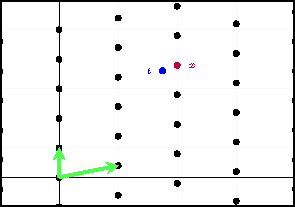
\includegraphics{figures/cvp.pdf}
				\end{figure}

				\begin{definition}[Bounded distance decoding (BDD)] \scriptsize Consider a basis $\basisB$, $\rho \in \RR^{+}$, and an $n$-dimensional lattice $\LL(\basisB)$. Given a vector $\vect \in \RR^{n}$ such that $\vect \notin \LL(\basisB)$, the \underline{bounded distance decoding} consists of finding the unique vector $\vecx \in \LL(\basisB)$ such that $\| \vect - \vecx \| \leq \rho$.
				\end{definition}

				\begin{itemize}
						\item The Goldreich-Goldwasser-Halevi is a nice introduction to the lattice concept of error-correction.
				\end{itemize}
\end{frame}

\begin{frame}{Motivation}{Goldreich-Goldwasser-Halevi cryptosystem (1997)}
				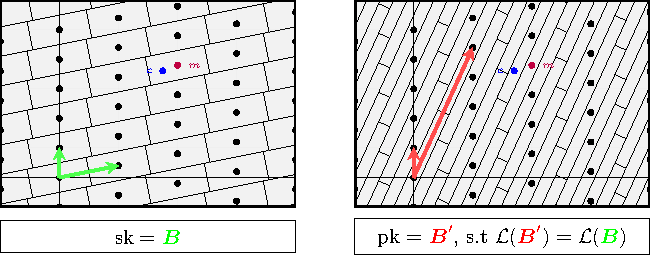
\includegraphics{figures/ggh-3.pdf}

				\begin{itemize}
								\justifying
								\item A {\color{green}\emph{good}} basis contains smaller and more orthogonal vectors.
								\item A {\color{red}\emph{bad}} basis contains larger and less orthogonal vectors.
								\item The cipher text $\color{blue}c$ is equal to the message ${\color{purple}m}$ plus a \underline{random small error}.
								\item Since the random error is \emph{small}, decrypting the message is equal to solving \BDD.
				\end{itemize}
\end{frame}


\begin{frame}{Motivation}{Babai`s nearest plane algorithm}
				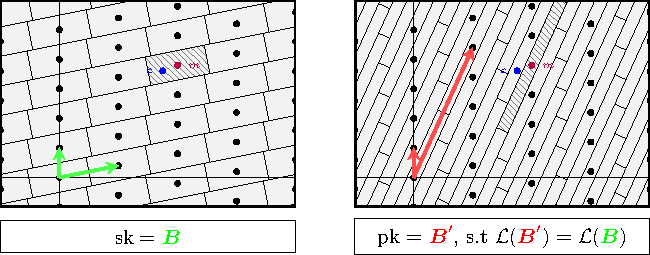
\includegraphics{figures/ggh-4.pdf}
								\begin{itemize}
												\justifying
												\item The $\textsc{Alg.}$ could be seen as partitioning the space $\RR^{n}$ with rectangles.
												\item Running the $\textsc{Alg.}$ with a \underline{bad} basis doesn't find the closest vector.
												\item BKZ is a basis reduction block-algorithm, having a blocksize $\beta$.
												\item A larger blocksize $\beta$ results on reduced bases with \underline{better quality}.
								\end{itemize}
\end{frame}


\begin{frame}{Motivation}{Babai`s nearest plane algorithm}
				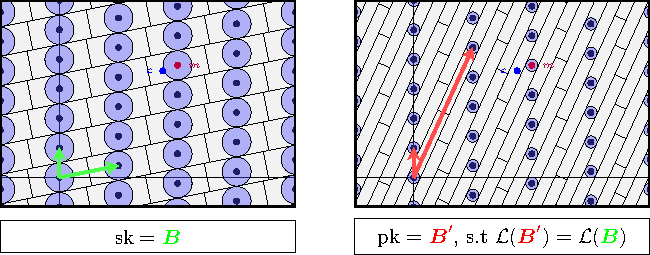
\includegraphics{figures/babai-decoding-radius.pdf}

				\begin{itemize}
								\item We denote the length of the largest error sampled in the encryption as $\rho$.
								\item Let $\Tilde{\basisB} = \textsc{GramSchmidt}(\basisB)$ denote the orthogonalized basis.
								\item The error correcting length of Babai's algorithm is defined by $\min_{\Tilde{\vecb} \in \Tilde{\basisB}}\{ \sfrac{\| \Tilde{\vecb} \|}{2} \}$.

				\end{itemize}
\end{frame}

\begin{frame}{Motivation}{When is decoding easy?}
				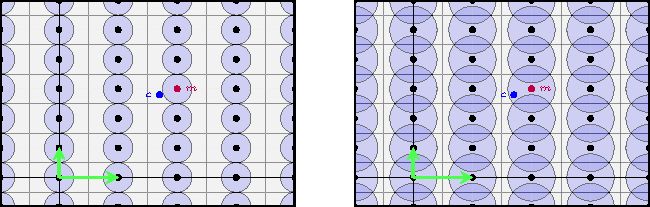
\includegraphics{figures/not-dense-lattice.pdf}

				\begin{definition}[Decoding gap]
							\justify{\fontfamily{roboto}\selectfont\scriptsize~The decoding gap of a lattice $\LL$ with decoding distance $\rho$ is defined as $\Gap_{\rho}(\LL) = \sfrac{\lambda_{1}}{\rho}$.}
				\end{definition}

				\begin{itemize}
								\justifying
								\item The largest length where vectors can be uniquely decoded is $\sfrac{\lambda_{1}}{2}$.
				\end{itemize}

				\myremark{A \underline{larger decoding gap} implies that the decoding problem can be \underline{solved by Babai's algorithm with a \emph{worst} basis}.}
\end{frame}

\begin{frame}{Motivation}{When is decoding easy?}
				\begin{figure}
								\centering
								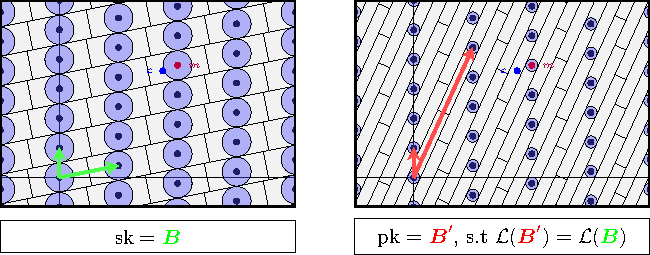
\includegraphics[scale=0.7]{figures/babai-decoding-radius.pdf}
				\end{figure}

				\myremark{Consider that each one of these cryptosystems have a \underline{\emph{system parameter}} named \underline{decoding length} $\rho$ and that all sampled errors $\vece$ have norm $\| \vece \| \leq \rho$.}

				\myheuristic{Most modern lattice-based cryptosystems are secure under the assumption that approximating solutions to BDD on an $n$-dimensional lattice $\LL$ with decoding distance $\rho$ and $\Gap_{\rho}(\LL) > \omega(\sqrt{n})$ is hard; and are broken by block reduction algorithms with blocksize $\beta < \sfrac{n}{2} + \littleO(n)$.}
\end{frame}

\begin{frame}
				\begin{figure}
								\Large How to improve lattice-based cryptosystems?
				\end{figure}

				\scriptsize R: Pick lattices with a small \underline{decoding gap} \dots, and use lattice isomorphism.
\end{frame}

\begin{frame}{Improving cryptosystems with isometries}
				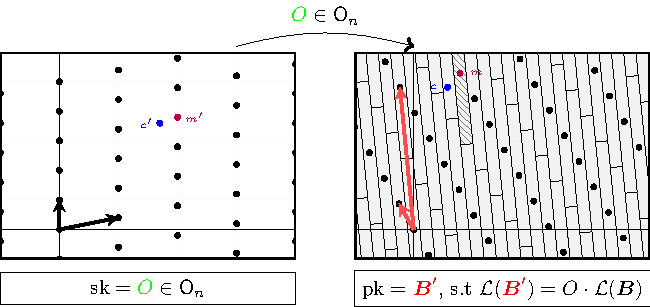
\includegraphics{figures/orthogonal-transformation.pdf}

				\myremark{The adversary and the recipient no longer have access to the same lattice.}

				\begin{itemize}
								\item Consider that we can efficiently decode erros in $\LL(\basisB)$.
				\end{itemize}
\end{frame}

\begin{frame}{Improving cryptosystems with isometries}
				\begin{figure}
								\centering
								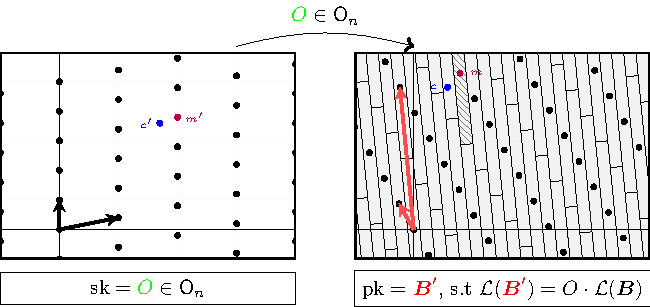
\includegraphics[scale=0.45]{figures/orthogonal-transformation.pdf}
				\end{figure}

				\mydefinition{Equivalent bases}{Let $\basisB$ and $\basisB'$ be two lattice basis. We say that both bases are equivalent and $\LL(\basisB) = \LL(\basisB')$ if there exists a unimodular transformation $U \in \UUn$ such that $\basisB' = \basisB \cdot U$.}

				\mydefinition{Lattice isomorphism}{Let $\LL$ and $\LL'$ be two lattices. We say that both lattices are isomorphic and $\LL \cong \LL'$ if there exists an orthogonal transformation $O \in \OOn$ such that $\LL' = O \cdot \LL$.}

				\mydefinition{Lattice isomorphism problem (LIP)}{Let $\basisB$ and $\basisB'$ be two lattice basis such that $\LL(\basisB) \cong \LL(\basisB')$. The LIP consists of finding an orthogonal transformation $O \in \OOn$ and a unimodular transformation $U \in \UUn$ such that $\basisB' = O \cdot \basisB \cdot U$.}
\end{frame}

\begin{frame}{Key-encapsulation mechanism}{Léo Ducas and van Woerden's frameworks}
				\begin{itemize}
								\item Léo Ducas and van Woerden's frameworks:
												\begin{itemize}
																\justifying
																\item Any lattice $\xrightarrow{}$ identification scheme;
																\item Decodable lattice $\xrightarrow{}$ (\sout{encryption}) key-encapsulation mechanism;
																\item A gaussian samplable lattice $\xrightarrow{}$ signature scheme.
								\end{itemize}

								\item Open problems:
												\begin{itemize}
																\justifying
																\item A concrete instance of a LIP-based key-encapsulation mechanism;
																\item \sout{A concrete instance of a LIP-based signature scheme};
																\item \sout{Investigate variations of LIP, such as Module-LIP};
																\item $\cdots$
												\end{itemize}
				\end{itemize}

				\begin{block}{Overall objectives}\scriptsize
								\begin{itemize}
												\justifying
												\item Review state-of-the art cryptoanalysis of LIP;
												\item present the current state of the art of modern cryptosystems having LIP as a foundation;
												\item propose a concrete instance of a LIP-based key-encapsulation mechanism.
												\item Investigate methods for improving our concrete KEM.
								\end{itemize}
				\end{block}
\end{frame}

\begin{frame}{Key-encapsulation mechanism}{Léo Ducas and van Woerden's frameworks}
		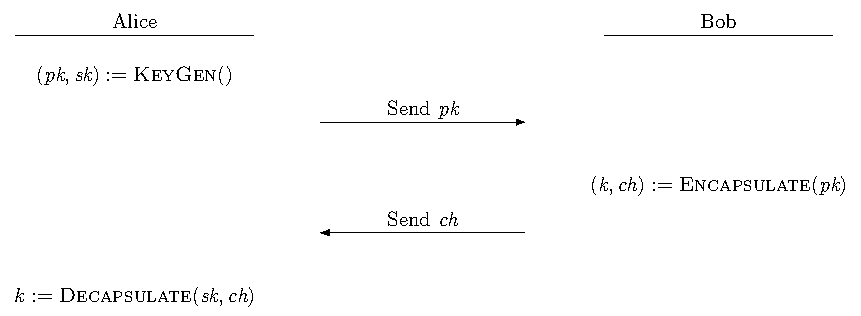
\includegraphics[scale=0.75]{figures/kem.pdf}

		\begin{definition}[KEM]
				A KEM is defined as having three algorithms named:
				\begin{itemize}\justifying
								\item key generation ($\textsc{KeyGen}$),
						\item encapsulation ($\textsc{Encapsulate}$),
						\item decapsulation ($\textsc{Decapsulate}$).
				\end{itemize}
		\end{definition}
\end{frame}

\begin{frame}{Key-encapsulation mechanism}{The framework}
				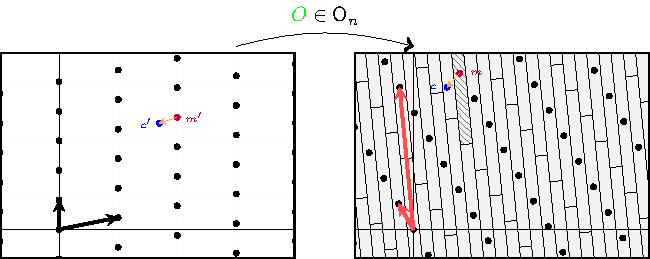
\includegraphics{figures/lip-based-kem.pdf}
				\myalgorithm{Encapsulation}{%
								\item Choose an arbitrary ${\color{purple}m}$.%
								\item Sample a random error $\vece$ such that $\| \vece \| \leq \rho = \sfrac{\lambda_{1}}{2}$.%
								\item Compute the vector ${\color{blue} \vecc} = {\color{purple}m} + \vece$.%
								\item Sample a random seed $\lambda$.%
								\item Sample a key $k = \mathcal{E}(\vece, \lambda)$ using the randomness extractor $\mathcal{E}$.%
								\item Return $(k, (\vecc, \lambda)) =$ \emph{shared secret} $\times$ encapsulated key.%
				}
\end{frame}

\begin{frame}{Key-encapsulation mechanism}{The framework}
				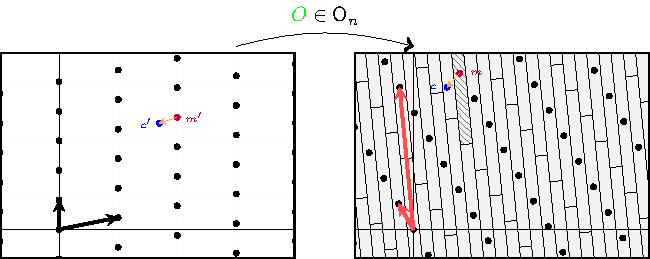
\includegraphics{figures/lip-based-kem.pdf}
				
				\myalgorithm{Decapsulation}{%
						\item Undo the rotation by computing ${\color{blue}\vecc'} = O^{-1} \cdot {\color{blue}\vecc}$.
						\item Decode the error as ${\color{purple}\vecm'} = \textsc{Decode}({\color{blue}\vecc'})$.
						\item Compute the erro vector $\vece' = {\color{blue}\vecc'} - {\color{purple}\vecm'}$.
						\item Rotate the error vector $\vece = O \cdot \vece'$.
						\item Extract a random shared key $k = \mathcal{E}(\vece, \lambda)$.
						\item Return $k$.
				}
\end{frame}


\begin{frame}{Key-encapsulation mechanism}{In practice, theory and practice are different}
				\uncover<1-4>{
								\begin{block}{Gram matrix}\scriptsize
												The gram matrix o a lattice basis $\basisB$ is a positive-defined quadratic form $Q = \basisB^{T} \basisB$.
								\end{block}
				}
				\uncover<2-4>{
								\begin{block}{Gram matrix of a rotated basis}\scriptsize
												\justify{Let $O \in \OOn$ be an orthogonal transformation. Note that the Gram matrix of a basis $\basisB' = O \cdot \basisB$ is equal to $Q' = (\basisB')^T (\basisB') = (O \cdot \basisB)^T (O \cdot \basisB) = \basisB^{T} O^{T} O \basisB = \basisB^T \basisB = Q$.}
								\end{block}
				}
				\uncover<3-4>{
								\begin{block}{Lattice isomorphism}\scriptsize
												\justify{Let $\basisB$ and $\basisB'$ be two bases having Gram matrices, respectivelly, $Q$ and $Q'$. The lattice $\LL(\basisB) \cong \LL(\basisB')$ if there exist a uniform matrix $U \in \UUn$ such that $Q' = U^{T} Q U $.}
								\end{block}
				}
				\uncover<4>{
								\myremark{
												\begin{itemize}
																\item \emph{In practice we use quadratic forms}.
																\item We can operate on the lattice vectors using quadratic forms and the integer coefficients. Consider $\vecv = \basisB \vecx$ and $\vecu = \basisB \vecy$, where $\vecx, \vecy \in \ZZ^{r}$.
																				\begin{enumerate}
																								\item $\langle \vecx, \vecy \rangle_{Q} = \vecx^{T} Q \vecy = \vecx^T \basisB^{T} \basisB \vecy = (\basisB \vecx)^{T} \basisB \vecy = \vecv^{T} \vecu = \langle \vecv, \vecu \rangle_{2}
																												$.
																								\item  $\| \vecx \|_{Q} = \sqrt{\vecx^{T} Q \vecx} = \sqrt{\langle \vecv, \vecv \rangle} = \| \vecv \|_{2}$.
																				\end{enumerate}
												\end{itemize}
								}
				}
\end{frame}

\begin{frame}{Key-encapsulation mechanism}{Practice}
				\begin{itemize}
								\item It is common among lattice-based KEMs to use SHA3-256 or SHA-256 as a randomness extractor.
												\begin{itemize}
																\item e.g. FrodoKEM, Crystal-Kyber.
																\item First encode the vector in binary, and then use SHA3-256, \ldots.
												\end{itemize}
				\end{itemize}


				\begin{example}
								Consider the basis $\basisB = [(11, 2), (-5, 1)]$ having Gram matrix $Q$ such that $\LL(\basisB) = \ZZ^{2}$. Let $\vecx = (5, 11)$, $\vecy = (10, 8)$ and $\vecz = (2, 40)$. If we encode $\vecy$ and $\vecz$ naively, the encoding is clearly not unique. Observe that

								\begin{itemize}
												\item $\vecy = (10, 8)$ would be encoded as $\overbrace{\boldsymbol{1010}}^{10}\overbrace{1000}^{8}$,
												\item $\vecz = (2, 40)$ would be encoded as $\overbrace{\boldsymbol{10}}^{2}\overbrace{101000}^{40}$;
								\end{itemize}

								and $\| \vecx \|_{Q} = \| \basisB \vecx \|_{2} = 1$ is very different from the norm $\| \vecx \|_{2} \geq 12 $.
				\end{example}
\end{frame}

\begin{frame}{Key-encapsulation mechanism}{Challenges and contributions}
				\begin{itemize}\setlength\itemsep{1em}
								\item Build a randomness-extractor for the real coefficients (because we use quadratic forms).
												\begin{enumerate}\setlength\itemsep{0.5em}
																\item Adapts Ajtai`s universal hash family to take as input small vectors considering the norm in respect to the quadratic forms.
																\item Build a randomness extractor from the unversal hash family using the Leftover hashing lemma.
												\end{enumerate}
								\item Handpick a \underline{decodable lattice} having a \underline{small decoding gap}.
								\item Build a lattice pair using the decodable lattice (IND-CPA).
								\item Then, $\ldots$
												\begin{figure}
																{\color{red} \large choose parameters so that all theorems are respected!}
												\end{figure}
				\end{itemize}
				\footnotetext{DOI: \href{https://doi.org/10.1109/ACCESS.2024.3358670}{10.1109/ACCESS.2024.3358670}}
\end{frame}

\begin{frame}{Spoiler alert!}

				\begin{table}[htbp]
								\centering
								\setlength{\tabcolsep}{3.2pt}
								\caption{Suggested parameter sets for our concrete KEM based on LIP.}\label{tab:parameters}
								\begin{tabular}{crrrrrrrr}
												\toprule
												Parameter set & $\LL$ & $\dim$ & $g$ & $\sim s$ & $q$ & $\hat{q}$ & $\hat{m}$ & $\beta$ \\
												\midrule
												OurBW256g2 & $\BW_{256}$ & $512$ & $2$ & $51$ & $3430$ & $880729$ & $12$ & $54880 \sqrt{2}$ \\
												OurBW512g2 & $\BW_{512}$ & $1024$ & $2$ & $75$ & $7479$ & $1431655751$ & $16$ & $239328$ \\
												OurBW256g4 & $\BW_{256}$ & $512$ & $4$ & $85$ & $2858$ & $880729$ & $12$ & $91456 \sqrt{2}$ \\
												OurBW512g4 & $\BW_{512}$ & $1024$ & $4$ & $125$ & $6233$ & $1431655751$ & $16$ & $398912$ \\
												OurBW256g8 & $\BW_{256}$ & $512$ & $8$ & $152$ & $2556$ & $880729$ & $12$ & $163584 \sqrt{2}$ \\
												OurBW512g8 & $\BW_{512}$ & $1024$ & $8$ & $225$ & $5610$ & $1431655751$ & $16$ & $718080$ \\
												OurBW256g12 & $\BW_{256}$ & $512$ & $12$ & $219$ & $2455$ & $880729$ & $12$ & $235680 \sqrt{2}$ \\
												OurBW512g12 & $\BW_{512}$ & $1024$ & $12$ & $325$ & $5402$ & $1431655751$ & $16$ & $1037184$ \\
												\bottomrule
								\end{tabular}
				\end{table}

				\uncover<2>{
								\begin{alertblock}{Important question}
												\Large Is this secure?
								\end{alertblock}
				}
\end{frame}

\begin{frame}{IND-CPA security}{Challenge}
				\begin{definition}[IND-CPA security] \scriptsize
								\justify{It is a security property common on encryption schemes, and key-encapsulation mechanisms. It is the concept that the advesary cannot \underline{distinguish a pair of ciphertexts given the message}. On KEMS, the adversary is unable to \underline{distinguish a pair of shared secrets, given the encapsulated key}.}
				\end{definition}

				\begin{block}{IND-CPA Challenge}
								\begin{enumerate}
												\item Let $(O, \basisB') := \textsc{KeyGen}(\basisB)$.
												\item Let $(k_{0}, (\vecc, \lambda)) := \textsc{Encaps}(\basisB')$.
												\item Let $k_{1} \xleftarrow{\$} \{0, 1\}^{l}$.
												\item Sample $b \xleftarrow{\$} \{0, 1\}$.
												\item Return to the adversary $(\basisB', (\vecc, \lambda), k_{b})$.
								\end{enumerate}

								\begin{itemize}
												\item The adversary wins the challenge if he can guess the value of $b$.
								\end{itemize}
				\end{block}
\end{frame}

\begin{frame}{IND-CPA security}{Why dense lattices?}
				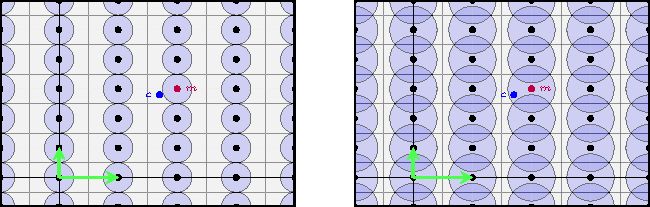
\includegraphics{figures/not-dense-lattice.pdf}

				\begin{block}{Overall idea}
								The idea is that the IND-CPA security challenge cannot be won when given a different lattice that is dense and has a much smaller decoding radius.
				\end{block}
\end{frame}

\begin{frame}{IND-CPA security}{Why dense lattices?}
				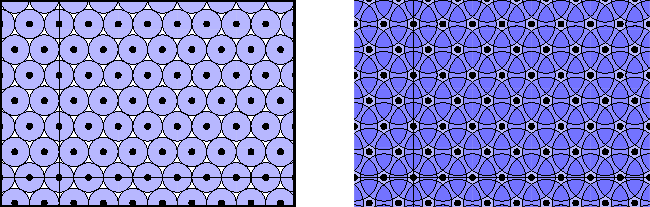
\includegraphics{figures/dense-lattice.pdf}
				\begin{block}{Overall idea}
								The idea is that the IND-CPA security challenge cannot be won when given a different lattice that is dense and has a much smaller decoding radius.
				\end{block}

\end{frame}


\begin{frame}{IND-CPA security}{Challenge}
				\begin{block}{IND-CPA Challenge}
								\begin{enumerate}
												\item Let $(O, \basisB') := \textsc{KeyGen}({\color{red}\basisB_{\textit{dense}}})$ ({\color{red} we replaced $\basisB$}).
												\item Let $(k_{0}, (\vecc, \lambda)) := \textsc{Encaps}(\basisB')$.
												\item Let $k_{1} \xleftarrow{\$} \{0, 1\}^{l}$.
												\item Sample $b \xleftarrow{\$} \{0, 1\}$.
												\item Return to the adversary $(\basisB', (\vecc, \lambda), k_{b})$.
								\end{enumerate}

								\begin{itemize}
												\item The adversary wins the challenge if he can guess the value of $b$.
								\end{itemize}
				\end{block}

				\begin{block}{$\Delta$ lattice isomorphism problem} Let $\basisB_{0}$ and $\basisB_{1}$ be two basis. Consider a random secret $b \in \{0, 1\}$ and a random public lattice $\LL \cong \LL(\basisB_{b})$. The $\DLIP$ consists of finding $b$.
				\end{block}

				\myremark{Theorem foundation: The KEM is IND-CPA secure under the assumption that solving $\DLIP(\basisB, \basisB_{\textit{dense}})$ is hard.}
\end{frame}


\begin{frame}{IND-CPA security}{Minimal example}
				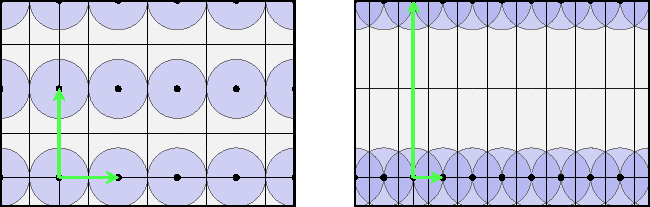
\includegraphics{figures/ind-cpa-challenge-2.pdf}
				\begin{example}
								Lattice pair example using $\LL(\basisB_{dense}) = \ZZ^{1}$, and $g = 2$.
								\begin{itemize}
												\item $\LL_{S} := g \cdot \LL(\basisB_{\textit{dense}}) \oplus (g+1) \cdot \LL(\basisB_{\textit{dense}}) = 2 \cdot \ZZ^{1} \oplus 3 \cdot \ZZ^{1}$
												\item $\LL_{Q} := \LL(\basisB_{\textit{dense}}) \oplus g (g + 1) \cdot \LL(\basisB_{\textit{dense}}) =  \ZZ^{1} \oplus 6 \cdot \ZZ^{1}$
								\end{itemize}
								Note that 
								\begin{itemize}
												\item $\lambda_{1}(\LL_{S}) = g \cdot \lambda_{1}(\LL(\basisB_{\textit{dense}}))$,
												\item and $\lambda_{1}(\LL_{Q}) = \lambda_{1}(\LL(\basisB_{\textit{dense}}))$.
								\end{itemize}
				\end{example}
\end{frame}


\begin{frame}{Parameters!}

				\begin{table}[htbp]
								\centering
								\setlength{\tabcolsep}{3pt}
								\begin{tabular}{crrrrrrrr}
												\toprule
												Parameter set & $\LL$ & $\dim$ & $g$ & $\sim s$ & $q$ & $\hat{q}$ & $\hat{m}$ & $\beta$ \\
												\midrule
												OurBW256g2 & $\BW_{256}$ & $512$ & $2$ & $51$ & $3430$ & $880729$ & $12$ & $54880 \sqrt{2}$ \\
												OurBW512g2 & $\BW_{512}$ & $1024$ & $2$ & $75$ & $7479$ & $1431655751$ & $16$ & $239328$ \\
												OurBW256g4 & $\BW_{256}$ & $512$ & $4$ & $85$ & $2858$ & $880729$ & $12$ & $91456 \sqrt{2}$ \\
												OurBW512g4 & $\BW_{512}$ & $1024$ & $4$ & $125$ & $6233$ & $1431655751$ & $16$ & $398912$ \\
												OurBW256g8 & $\BW_{256}$ & $512$ & $8$ & $152$ & $2556$ & $880729$ & $12$ & $163584 \sqrt{2}$ \\
												OurBW512g8 & $\BW_{512}$ & $1024$ & $8$ & $225$ & $5610$ & $1431655751$ & $16$ & $718080$ \\
												OurBW256g12 & $\BW_{256}$ & $512$ & $12$ & $219$ & $2455$ & $880729$ & $12$ & $235680 \sqrt{2}$ \\
												OurBW512g12 & $\BW_{512}$ & $1024$ & $12$ & $325$ & $5402$ & $1431655751$ & $16$ & $1037184$ \\
												\bottomrule
								\end{tabular}
				\end{table}

				\uncover<1>{
								\myremark{Important answer: The KEM is IND-CPA secure under the assumption that solving $\DLIP$ is hard.}
				}
\end{frame}

\begin{frame}{Our work in perspective}{Key sizes (IND-CPA)}

				\begin{table}[htbp]
								\centering
								\small
								\setlength{\tabcolsep}{5pt}
								\begin{tabular}{crrrrrrc}
												\toprule
												IND-CPA KEM & & & & & & & \\
												\midrule
												Parameter set & $|\pk|$ & $|\sk|$ & $|\ch|$ & $|\ss|$ & $\beta$ & $\lambda$ \\
												\midrule
												OurBW256g2 & $ 439.25$ KB & $384$ KB & $ 781.88$ B & $240$ b & $352$ & $2^{111}$ \\
												OurBW512g2 & $ 1.91$ MB & $ 1.62$ MB & $ 1.65$ KB & $496$ b & $700$ & $2^{213}$ \\
												OurBW256g4 & $ 463.18$ KB & $384$ KB & $ 778.62$ B & $240$ b & $265$ & $2^{85}$ \\
												OurBW512g4 & $ 2.00$ MB & $ 1.62$ MB & $ 1.65$ KB & $496$ b & $557$ & $2^{171}$ \\
												OurBW256g8 & $ 489.93$ KB & $416$ KB & $ 776.25$ B & $240$ b & $201$ & $2^{66}$ \\
												OurBW512g8 & $ 2.11$ MB & $ 1.75$ MB & $ 1.64$ KB & $496$ b & $449$ & $2^{139}$ \\
												OurBW256g12 & $ 506.89$ KB & $448$ KB & $ 775.12$ B & $240$ b & $173$ & $2^{57}$ \\
												OurBW512g12 & $ 2.17$ MB & $ 1.88$ MB & $ 1.64$ KB & $496$ b & $398$ & $2^{124}$ \\
												\bottomrule
								\end{tabular}
				\end{table}
\end{frame}


\begin{frame}{Our work in perspective}{Key sizes (IND-CCA2)}

				\begin{table}[htbp]
								\centering
								\setlength{\tabcolsep}{2.7pt}
								\begin{tabular}{crrrrrrc}
												\toprule
												IND-CCA2 KEM & & & & & & & \\
												\midrule
												Parameter set & $|\pk|$ & $|\sk|$ & $|\ch|$ & $|\ss|$ & $\beta$ \\
												\midrule	
												OurBW256g2 & $ 439.25$ KB & $ 384.01$ KB & $ 797.88$ B & $111$ b & $352$ & $2^{111}$ \\
												OurBW512g2 & $ 1.91$ MB & $ 1.63$ MB & $ 1.68$ KB & $213$ b & $700$ & $2^{213}$ \\
												OurBW256g4 & $ 463.18$ KB & $ 384.01$ KB & $ 794.62$ B & $85$ b & $265$ & $2^{85}$ \\
												OurBW512g4 & $ 2.00$ MB & $ 1.63$ MB & $ 1.68$ KB & $171$ b & $557$ & $2^{171}$ \\
												OurBW256g8 & $ 489.93$ KB & $ 416.01$ KB & $ 792.25$ B & $66$ b & $201$ & $2^{66}$ \\
												OurBW512g8 & $ 2.11$ MB & $ 1.75$ MB & $ 1.67$ KB & $139$ b & $449$ & $2^{139}$ \\
												OurBW256g12 & $ 506.89$ KB & $ 448.01$ KB & $ 791.12$ B & $57$ b & $173$ & $2^{57}$ \\
												OurBW512g12 & $ 2.17$ MB & $ 1.88$ MB & $ 1.66$ KB & $124$ b & $398$ & $2^{124}$ \\
												\bottomrule
								\end{tabular}
				\end{table}

				\myremark{We converted the IND-CPA secure KEM to an IND-CCA2 secure KEM using well-known methods described in the literature, including the transformation of Fujisaki-Okamoto.}
\end{frame}

\begin{frame}{Our work in perspective}{Modern lattice-based KEMs}

				\begin{table}[htbp]
								\centering
								\setlength{\tabcolsep}{10pt}
								\begin{tabular}{crrrr}
												\toprule
												Parameter set & $|\pk|$ & $\lambda$ \\
												\midrule \small
												% LOTUS
												lotus-params128 & $658.95$ KB & $2^{196}$ \\
												lotus-params192 & $1.00$ MB & $2^{199}$ \\
												% FrodoKEM
												Frodo-640 & $9.39$ KB & $2^{149}$ \\
												Frodo-976 & $15.26$ KB & $2^{214}$ \\ 
												NewHope512 & 928 B & $2^{112}$ \\
												Kyber512 & $800$ B & $2^{118}$ \\
												Kyber768 & $1.15$ KB & $2^{182}$ \\
												% LightSaber & pk & sk & ch & block & SVP & -- \\
												% FireSaber & pk & sk & ch & block & SVP & -- \\
												% Saber & pk & sk & ch & block & SVP & -- \\
												% NTRU Prime
												% Lizard
												KEM\_CATEGORY1\_N536 & $1.07$ MB & $2^{133}$ \\
												KEM\_CATEGORY3\_N816 & $1.64$ MB & $2^{193}$ \\
												% EMBLEM
												% Titanium
												Titanium-CCA-Std128 & $14.37$ KB & $2^{146}$ \\
												Titanium-CCA-Med160 & $16.06$ KB & $2^{192}$ \\
												\bottomrule
								\end{tabular}
				\end{table}
\end{frame}

\begin{frame}{Our work in perspective}{Conclusion}
				\myremark{It is easier to study specific optimizations once we have a first concrete instance.}

				\begin{block}{Overall objectives} \scriptsize
								\begin{itemize}
												\justifying
												\item<2-3> Review state-of-the art cryptoanalysis of LIP $\bcancel{\checkmark}$;
												\item<2-3> present the current state of the art of modern cryptosystems having LIP as a foundation $\bcancel{\checkmark}$;
												\item<1-3> propose a concrete instance of a LIP-based key-encapsulation mechanism \checkmark;
												\item<3-> Investigate methods for improving our concrete KEM.
								\end{itemize}
				\end{block}
\end{frame}

\begin{frame}{Open questions}{Sublattice isomorphism}
				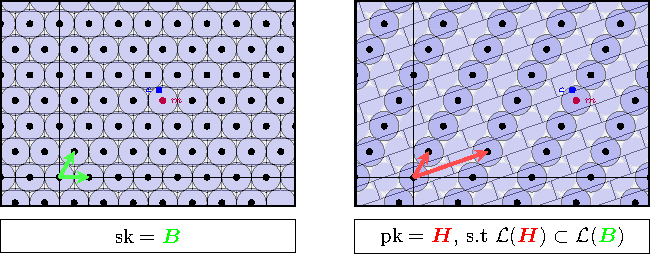
\includegraphics{figures/working-with-sublattices.pdf}

				\begin{itemize}
								\item In our example, the rank of $\LL(\basisH)$ and $\LL(\basisB)$ are the same.
								\item The same idea could be applied to the LIP Framework.
								\item However, the lattices are no longer isomorphic. For some $\LL$, \[\LL(\basisB') \subset \LL \cong \LL(\basisB).\]
								\item Similar ideas exists in code-based cryptography, e.g subcode equivalence problem.
				\end{itemize}
\end{frame}

\end{document}
